% =====================================================================
%  Prabhavit Gupta - Tailored CV for AI Automation Specialist
%  Target: Bamboo Works (AI-Powered Accounting & Bookkeeping Systems)
%  Role: AI Automation Specialist (Claude & Accounting Workflows)
%  Compile: tectonic cv/main_BambooWorks_AIAutomation.tex
%  Rules: ONE PAGE. No unicode em-dashes. Plain voice. Verified facts. ATS-optimized.
% =====================================================================
\documentclass[a4paper,10pt]{article}

\usepackage[T1]{fontenc}
\usepackage[utf8]{inputenc}
\usepackage[top=0.7cm,bottom=0.7cm,left=1.0cm,right=1.0cm]{geometry}
\usepackage{titlesec}
\usepackage{enumitem}
\usepackage{hyperref}
\usepackage{xcolor}
\usepackage{graphicx}

\definecolor{accent}{HTML}{1F4E78}
\hypersetup{colorlinks=true, urlcolor=accent, linkcolor=accent}
\pagestyle{empty}
\setlength{\parindent}{0pt}

\titleformat{\section}{\large\bfseries\color{accent}}{}{0em}{}[\vspace{-0.6em}\rule{\textwidth}{0.8pt}]
\titlespacing{\section}{0pt}{2pt}{1pt}

\newcommand{\role}[4]{%
  \textbf{#1} \hfill \textbf{#2}\\[1pt]%
  \textit{#3} \hfill \textit{#4}\\[2pt]%
}
\setlist[itemize]{leftmargin=1.2em, itemsep=0pt, topsep=1pt, parsep=0pt}

\begin{document}

% ================= HEADER =================
\begin{minipage}[c]{0.80\textwidth}
  {\Huge\bfseries Prabhavit Gupta}\\[3pt]
  {\color{accent}\large AI Automation Specialist: Claude Agents, Document Pipelines \& Integrations}\\[5pt]
  {\footnotesize +39 351 610 7807 ~$\vert$~
  \href{mailto:prabhavitg@gmail.com}{prabhavitg@gmail.com} ~$\vert$~
  \href{https://www.linkedin.com/in/prabhavit/}{linkedin.com/in/prabhavit} ~$\vert$~
  \href{https://github.com/prab-gupta}{github.com/prab-gupta} ~$\vert$~
  Venice, Italy}
\end{minipage}\hfill
\begin{minipage}[c]{0.18\textwidth}
  \raggedleft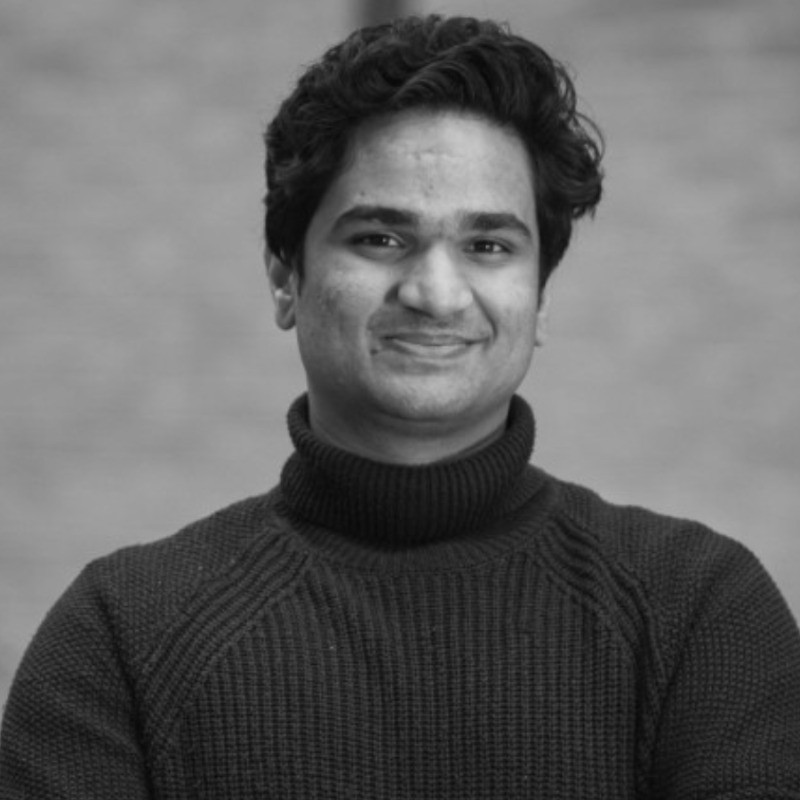
\includegraphics[width=2.0cm]{photo.jpg}
\end{minipage}
\vspace{-2pt}

% ================= SUMMARY =================
\section{Summary}
AI Automation Specialist with 3+ years of experience engineering production LLM agents, document parsing workflows, and system integrations using Claude, Claude Code, Python, and TypeScript. At FlowSpace, built multi-format document extraction pipelines (PDF, web, image, spreadsheet to validated JSON), autonomous support agents with confidence-based human escalation, and billing/booking API integrations on a live platform. Holds an academic background in Economics, combining practical agent orchestration and workflow design with a natural understanding of accounting logic, financial reconciliation, and exception handling.

% ================= SKILLS =================
\section{Skills}
\begin{itemize}
  \item \textbf{AI Agents, Claude \& Orchestration:} Claude and Claude Code, Anthropic API, multi-agent workflows, prompt engineering and chaining, RAG architectures, confidence scoring, audit trails, human-in-the-loop review, agent evaluation and failure recovery
  \item \textbf{Accounting \& Workflow Automation:} Receipt and invoice data extraction, unstructured document parsing into validated JSON schemas, transaction categorization, RFI workflows, n8n, Make, event-driven pipelines, automated reconciliation logic
  \item \textbf{Full-Stack, APIs \& Platforms:} Python, TypeScript, Node.js, Next.js, Laravel (PHP), REST APIs, webhooks, Supabase, PostgreSQL, MySQL, Docker, Playwright, Git; familiar with accounting platforms (Xero, QuickBooks, Zoho, Odoo) and CRM/billing integrations
\end{itemize}

% ================= EXPERIENCE =================
\section{Experience}

\role{\href{https://flowspace.co}{FlowSpace.co}}{Mar 2024 -- Aug 2026}{Lead Developer \& AI Automation Engineer (Full-time, Freelance)}{London, UK (remote)}
\begin{itemize}
  \item Architected and deployed an end-to-end AI document ingestion pipeline (n8n, Claude API, TypeScript) extracting unstructured data from PDF, spreadsheet, image, and web brochures into validated backend schemas with human review; 900+ entities processed.
  \item Shipped customer-facing AI agents operating over live platform data, incorporating confidence scoring thresholds and automated escalation to human support for ambiguous inquiries.
  \item Engineered REST API and webhook integrations with OfficeRnD and Nexudus for automated booking synchronization, billing schedules, and financial record consistency across platforms.
  \item Led platform and database migration off a legacy stack to modern Next.js and Laravel (PostgreSQL), scaling from 2,000 to 4,500+ users without downtime, alongside CRM lead capture and routing automations.
\end{itemize}

\role{\href{https://ultrastrategy.com}{UltraStrategy.com}}{Dec 2024 -- May 2025}{AI Automation Developer (Collaborator)}{France (remote)}
Built an automated LLM document extraction pipeline in n8n and Eden AI, parsing unstructured documents into normalized, schema-validated JSON records across multi-tier user profiles.\\[1pt]

\role{\href{https://get2germany.com}{Get2Germany.com}}{Jan 2024 -- May 2024}{Developer \& Automation Specialist (Part-time)}{Berlin, Germany (remote)}
Built automated data collection and validation pipelines using n8n and Google APIs, streamlining database updates and candidate matching logic.\\[1pt]

\role{\href{https://clubee.com}{Clubee.com}}{Sep 2023 -- Aug 2024}{Developer \& QA (Full-time, Freelance)}{Foetz, Luxembourg (remote)}
Integrated core REST APIs across frontend modules, executed comprehensive QA/unit testing, and delivered administrative dashboards.

% ================= PROJECTS =================
\section{Selected Projects}
\begin{itemize}
  \item \textbf{\href{https://github.com/prab-gupta/llm-doc-parser}{LLM Document Parser}} (\href{https://github.com/prab-gupta/llm-doc-parser}{github.com/prab-gupta/llm-doc-parser}): Open-source engine demonstrating multi-format document parsing (PDF, image, text) into strictly typed, validated JSON structures with automated error recovery.
  \item \textbf{\href{https://smarturlink.com/}{Urlink}} (2025): Project Manager \& AI Developer; built client requirements, platform logic, and automated workflows using Next.js and Supabase.
\end{itemize}

% ================= EDUCATION \& CERTIFICATIONS =================
\section{Education \& Certifications}
\textbf{Ca' Foscari University of Venice} \hfill Oct 2020 -- Jun 2024\\
BA Philosophy, International Studies \& Economics (Minor: Entrepreneurship)\\[1pt]
\textbf{Certifications:} Microsoft Copilot Studio Agent Academy \textbullet\ Microsoft: Building AI Agents \textbullet\ Microsoft Power Automate \textbullet\ Tray.AI Build Practitioner

% ================= WORK AUTHORIZATION =================
\vspace{2pt}
{\small \textbf{Work authorization:} Italian EU Long Term Residence Permit (independent contractor / Partita IVA). Available immediately. Fully flexible with Australian business hours. \quad \textbf{Languages:} English (fluent C2), Hindi (native), Italian (conversational).}

\end{document}
